Setelah seluruh komponen sistem navigasi diimplementasikan dan diintegrasikan ke dalam lingkungan simulasi, tahap berikutnya adalah melakukan pengujian untuk mengevaluasi pengaruh integrasi kamera termal dan pengendali fuzzy terhadap performa navigasi robot. Pengujian dirancang untuk merepresentasikan berbagai kondisi lingkungan yang umum dijumpai pada navigasi robot bergerak di area dalam ruangan, mulai dari lingkungan tanpa obstacle hingga lingkungan dengan obstacle dinamis.

\subsection{Tujuan Pengujian}

Pengujian dilakukan untuk mengevaluasi kemampuan sistem dalam mendeteksi obstacle pada area blind-spot LiDAR, menghindari obstacle statis maupun dinamis, serta mencapai tujuan navigasi secara aman dan efisien.

Secara khusus, pengujian bertujuan untuk:

\begin{enumerate}
\item Mengevaluasi kemampuan integrasi LiDAR dan kamera termal dalam meningkatkan per\-sepsi lingkungan.
\item Menganalisis pengaruh pengendali fuzzy terhadap perilaku navigasi robot.
\item Membandingkan performa sistem baseline dan sistem fuzzy pada kondisi lingkungan yang identik.
\item Mengukur stabilitas dan keamanan navigasi pada berbagai skenario obstacle.
\end{enumerate}

\subsection{Konfigurasi Skenario Pengujian}

Eksperimen dilakukan menggunakan delapan skenario yang dibagi menjadi dua kelompok, yaitu kelompok baseline dan kelompok fuzzy. Seluruh skenario menggunakan peta, robot, dan konfigurasi sensor yang sama sehingga perbedaan performa yang diamati hanya dipengaruhi oleh mekanisme pengendalian yang digunakan.

Tabel~\ref{tab:skenario_pengujian} menunjukkan konfigurasi skenario yang digunakan.

\begin{table}[H]
\centering
\caption{Skenario pengujian yang digunakan}
\label{tab:skenario_pengujian}
\begin{tabular}{cccc}
\toprule
\textbf{Skenario} &
\textbf{Kelompok} &
\textbf{Kondisi Lingkungan} &
\textbf{Fuzzy} \\
\midrule
S1 & Baseline & Tanpa obstacle & Tidak \\
S2 & Baseline & Satu obstacle manusia & Tidak \\
S3 & Baseline & Multiple obstacle statis & Tidak \\
S4 & Baseline & Multiple obstacle dinamis & Tidak \\
S5 & Fuzzy & Tanpa obstacle & Ya \\
S6 & Fuzzy & Satu obstacle manusia & Ya \\
S7 & Fuzzy & Multiple obstacle statis & Ya \\
S8 & Fuzzy & Multiple obstacle dinamis & Ya \\
\bottomrule
\end{tabular}
\end{table}

\subsubsection*{a. Skenario S1/S5 --- Navigasi Tanpa Obstacle}

Skenario S1 dan S5 menggunakan lingkungan \texttt{S1\_open.world} yang tidak mengandung obstacle aktif selain dinding dan struktur peta statis. Skenario ini berfungsi sebagai \textit{control condition} untuk mengisolasi efek logika fuzzy terhadap pola navigasi robot pada kondisi bebas gangguan. Pada S5, \textit{fuzzy controller} aktif meskipun tidak ada obstacle terdekat, sehingga $d_\text{obs}$ selalu tinggi dan $\tau_\text{eff} \approx 1{,}0$; sesuai basis aturan, robot diizinkan bergerak dengan kecepatan penuh dan gain lemah. Selisih kecepatan dan panjang lintasan antara S1 dan S5 menjadi indikator \textit{overhead} yang ditimbulkan fuzzy pada kondisi normal.

\subsubsection*{b. Skenario S2/S6 --- Satu Obstacle Statis}

Skenario S2 dan S6 menggunakan lingkungan \texttt{S2\_single\_human.world} yang memuat satu \textit{obstacle} manusia statis (silinder $r = 0{,}25$~m, tinggi 3~m, posisi $(2{,}466;\ 1{,}273)$~m) yang dapat dideteksi oleh LiDAR. Skenario ini menguji kemampuan dasar penghindaran \textit{obstacle} konvensional serta efek logika fuzzy terhadap \textit{clearance} pada kondisi \textit{obstacle} tunggal. Tidak terdapat \textit{obstacle} kucing pada skenario ini.

\subsubsection*{c. Skenario S3/S7 --- Obstacle Majemuk Statis dengan Kucing}

Skenario S3 dan S7 merupakan skenario utama yang menguji hipotesis penelitian, yaitu apakah sistem mampu menghindari \textit{obstacle} kucing yang tidak terdeteksi LiDAR. Lingkungan \texttt{S3\_static\_multi.world} memuat tiga \textit{obstacle} statis, yaitu: (a) satu \textit{obstacle} statis standar ($r = 0{,}25$~m), (b) \texttt{obstacle\_cat} ($r = 0{,}18$~m, tinggi $\approx$0,19~m, posisi $(2{,}83;\ 0{,}97)$~m) yang berada di \textit{blind-spot} LiDAR, dan (c) dua \textit{obstacle\_human} statis ($r = 0{,}25$~m, tinggi 3~m). Pasangan S3/S7 memungkinkan perbandingan \textit{clearance} terhadap kucing antara konfigurasi \textit{baseline} dan fuzzy dalam kondisi yang terkontrol.

\subsubsection*{d. Skenario S4/S8 --- Obstacle Majemuk Dinamis dengan Kucing}

Skenario S4 dan S8 menambahkan lapisan kompleksitas dengan menggerakkan kedua \textit{obstacle} manusia secara osilasi mulus menggunakan skrip \texttt{dynamic\_obstacles.py}. Masing-masing \textit{obstacle} manusia bergerak bolak-balik di sepanjang jalur linear: human\_1 menempuh jalur sepanjang $\approx 3{,}07$~m dan human\_2 sepanjang $\approx 3{,}23$~m, keduanya dengan profil kecepatan sinusoidal yang menghasilkan kecepatan puncak masing-masing $\approx 0{,}77$~m/s dan $\approx 0{,}81$~m/s. Gerak osilasi dimodelkan menggunakan fungsi:
\begin{equation}
    s(t) = \frac{1}{2}\bigl(1 - \cos(\omega t)\bigr),
    \quad \omega = 0{,}5~\text{rad/s}
    \label{eq:osilasi_human}
\end{equation}
di mana $s(t) \in [0, 1]$ adalah parameter posisi ternormalisasi di sepanjang jalur masing-masing \textit{obstacle} ($s=0$: titik A, $s=1$: titik B). Fungsi kosinus terbalik ini menghasilkan gerakan yang halus dengan akselerasi dan deselerasi di kedua ujung jalur, sehingga menghindari perubahan kecepatan mendadak yang tidak realistis. Posisi \textit{obstacle} diperbarui melalui layanan \texttt{/gazebo/set\_model\_state} pada frekuensi 50~Hz.

Fase gerak \textit{obstacle} tidak direset antar-\textit{trial}, sehingga setiap \textit{trial} mengalami kondisi pertemuan yang berbeda dan lebih mendekati variasi alami yang diharapkan pada penerapan nyata. Posisi kucing (\texttt{obstacle\_cat}) pada S4 terdapat sedikit \textit{offset} dibandingkan S3 ($\Delta x \approx 0{,}14$~m, $\Delta y \approx 0{,}003$~m) karena perbedaan \textit{world file}, tetapi perbedaan ini tidak mengubah karakteristik \textit{blind-spot}-nya secara substansial.

Pada skenario S4 dan S8, mekanisme \textit{dynamic prediction} dan \textit{temporal yield} juga aktif, sebagai respons terhadap karakteristik \textit{obstacle} yang bergerak dengan kecepatan mendekati 0,8~m/s. Parameter APF yang berbeda dari skenario lain ($d_0 = 1{,}20$~m, \texttt{obs\_detect\_radius} = 1,30~m) juga hanya berlaku pada S4 dan S8 untuk memberikan jarak reaksi yang lebih awal terhadap \textit{obstacle} dinamis.

\begin{figure}[H]
    \centering
    \begin{minipage}{0.48\textwidth}
        \centering
        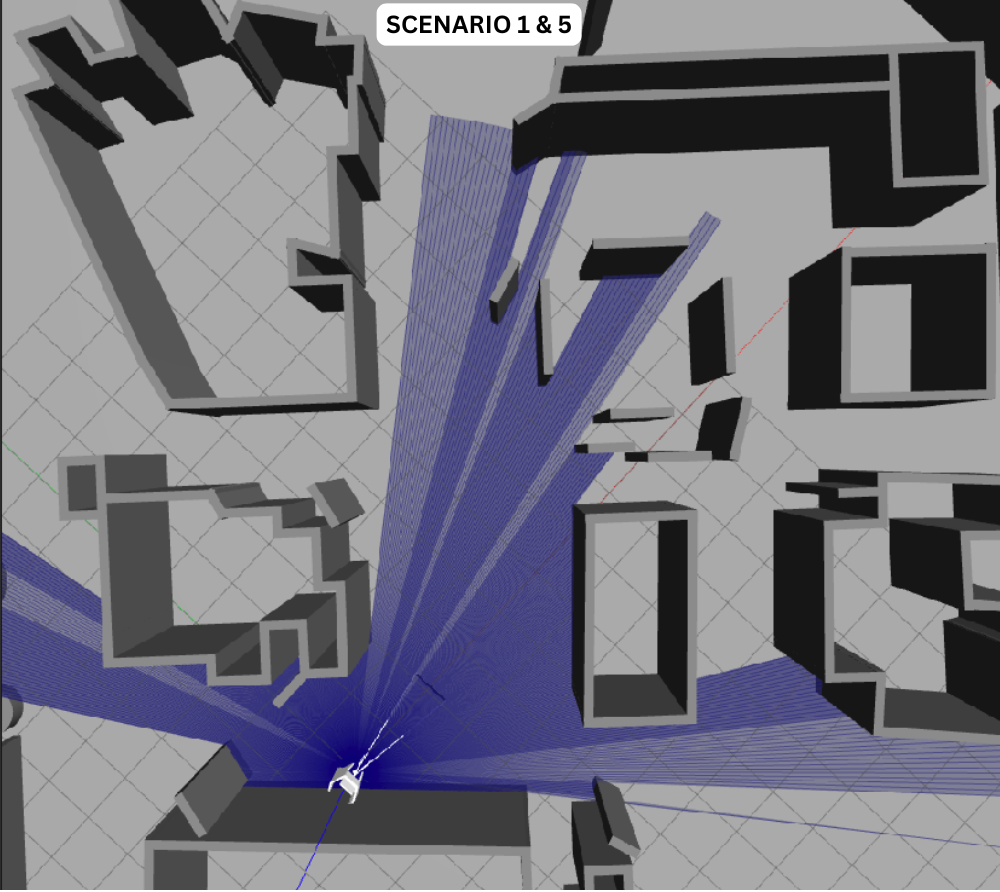
\includegraphics[width=\textwidth]{gambar/3.8_skenario_S1_S5.png}
        \\(a) S1/S5
    \end{minipage}
    \hfill
    \begin{minipage}{0.48\textwidth}
        \centering
        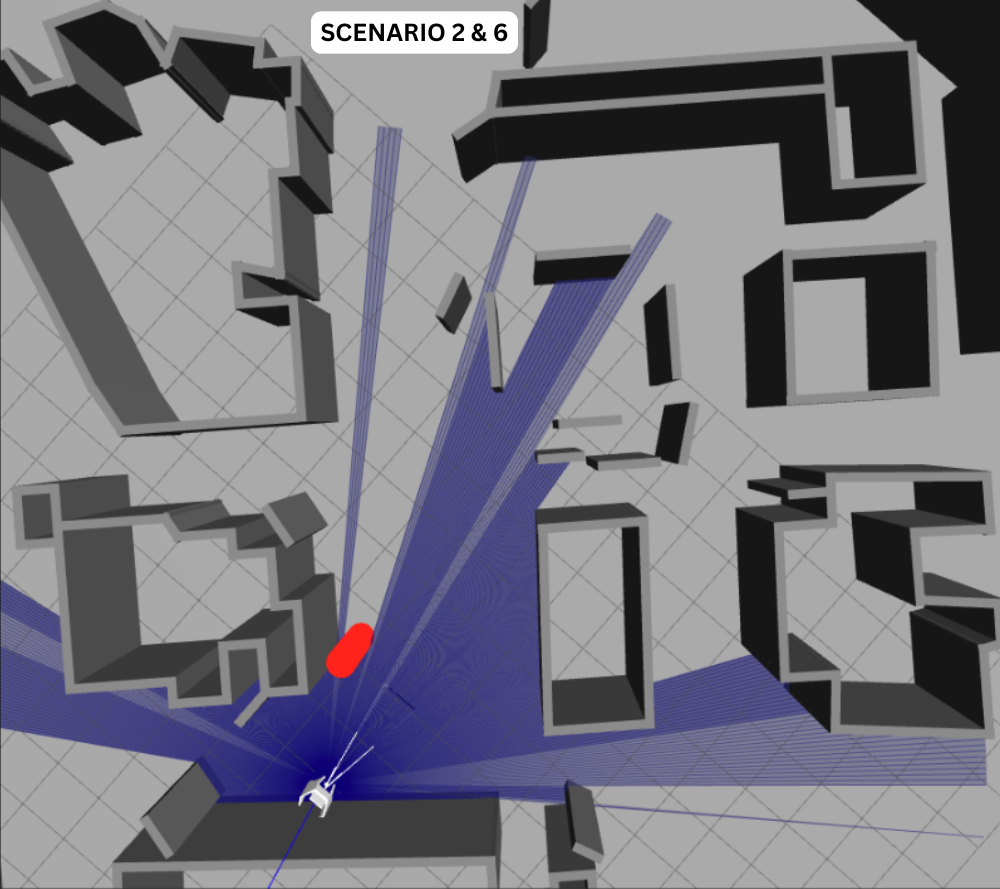
\includegraphics[width=\textwidth]{gambar/3.8_skenario_S2_S6.png}
        \\(b) S2/S6
    \end{minipage}

    \vspace{0.5em}

    \begin{minipage}{0.48\textwidth}
        \centering
        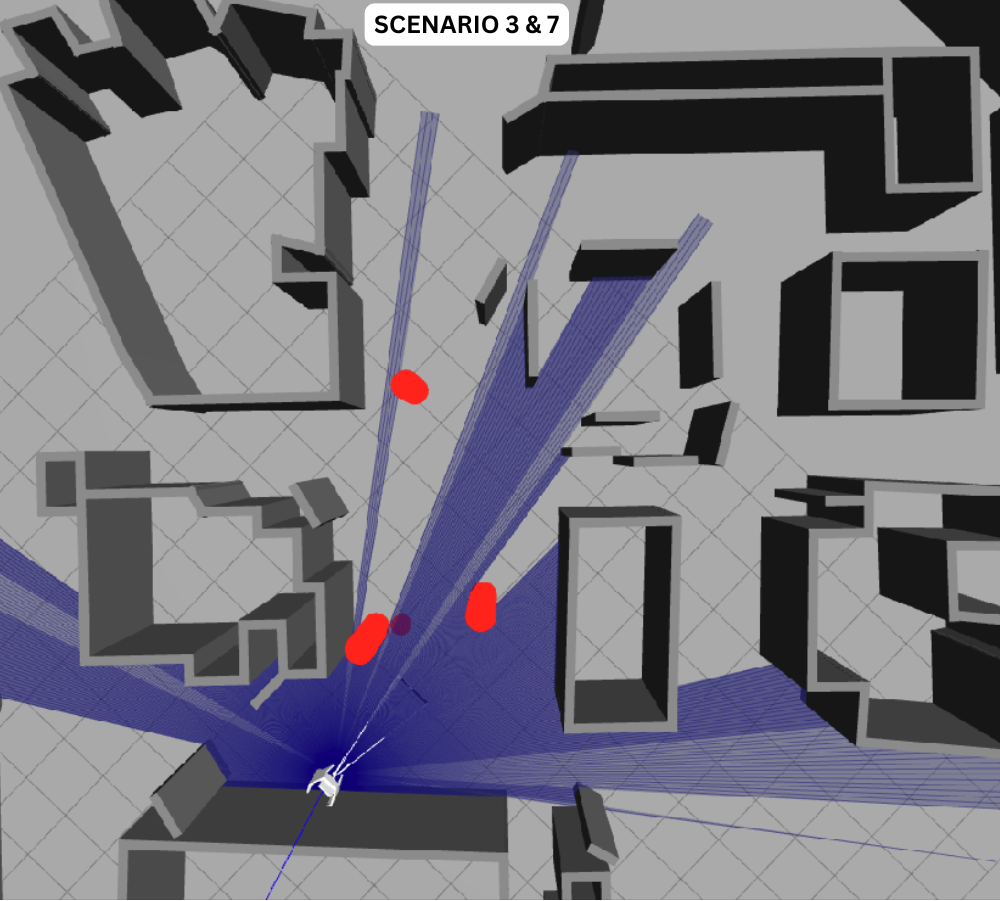
\includegraphics[width=\textwidth]{gambar/3.8_skenario_S3_S7.png}
        \\(c) S3/S7
    \end{minipage}
    \hfill
    \begin{minipage}{0.48\textwidth}
        \centering
        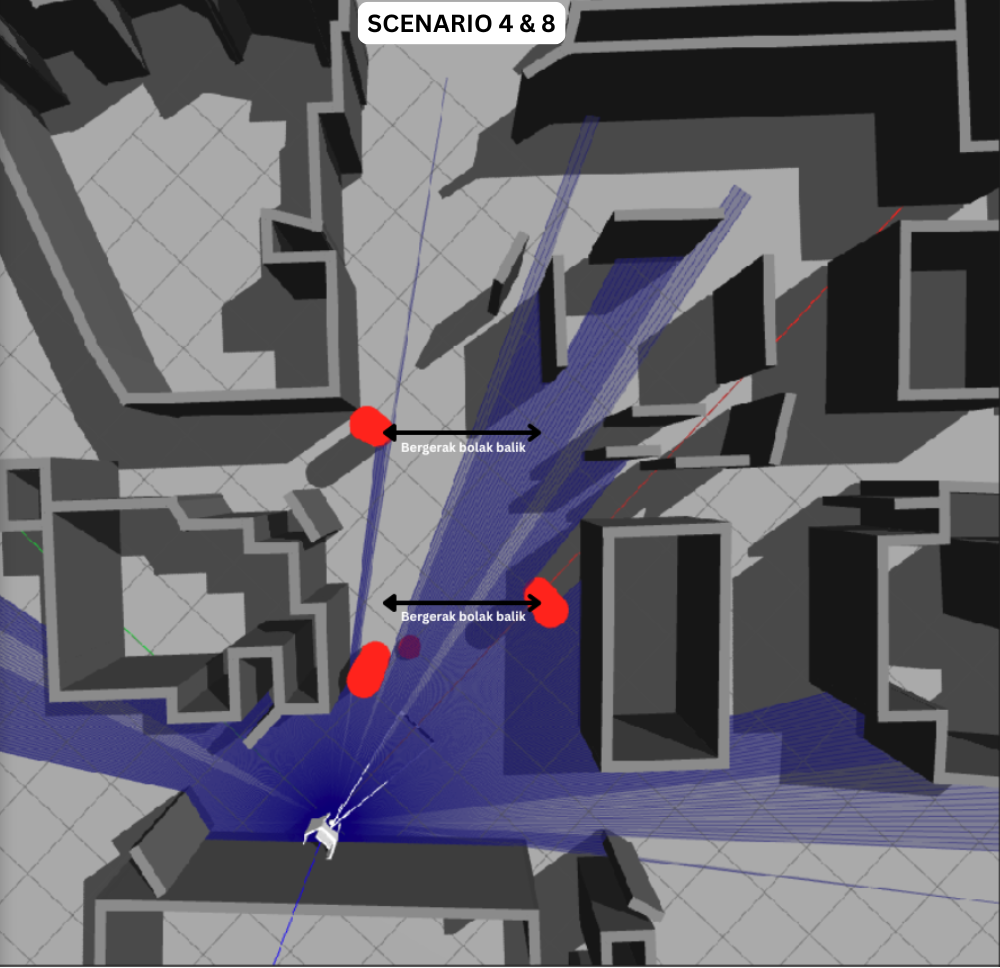
\includegraphics[width=\textwidth]{gambar/3.8_skenario_S4_S8.png}
        \\(d) S4/S8
    \end{minipage}
    \caption{Tampak atas empat lingkungan pengujian di Gazebo. Jalur biru menunjukkan jangkauan pindaian LiDAR \textit{real-time}; blob merah menandai sumber panas yang terdeteksi kamera termal. (a) S1/S5: tanpa \textit{obstacle} aktif. (b) S2/S6: satu \textit{obstacle} statis bersuhu tubuh. (c) S3/S7: tiga sumber panas (\textit{obstacle\_cat} dan dua \textit{obstacle\_human}) dari total empat \textit{obstacle} fisik; satu \textit{obstacle} statis tambahan tidak terdeteksi termal karena tidak bersuhu tubuh. (d) S4/S8: dua \textit{obstacle\_human} bergerak osilasi (ditandai panah \textit{"Bergerak bolak balik"}), sedangkan \textit{obstacle\_cat} tetap statis.}
    \label{fig:skenario_panel}
\end{figure}

\begin{figure}[H]
    \centering
    \begin{minipage}{0.48\textwidth}
        \centering
        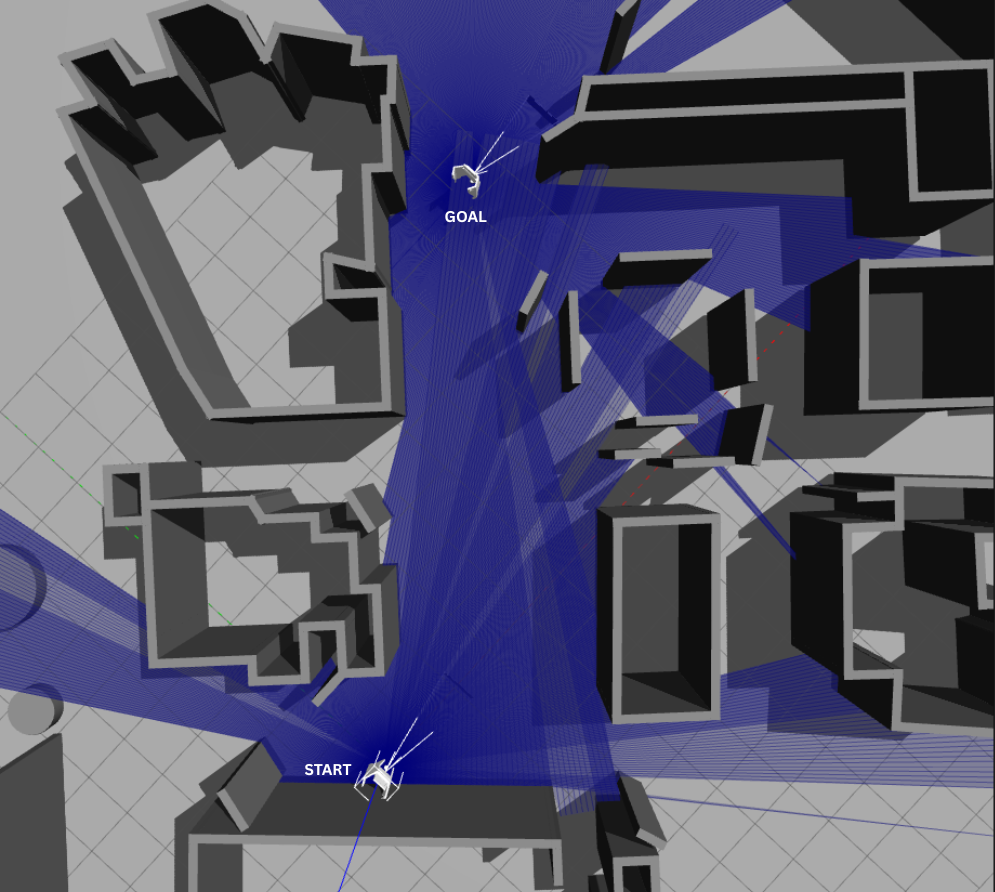
\includegraphics[width=\textwidth]{gambar/3.8_map_gazebo.png}
        \\(a) Tampak atas Gazebo
    \end{minipage}
    \hfill
    \begin{minipage}{0.48\textwidth}
        \centering
        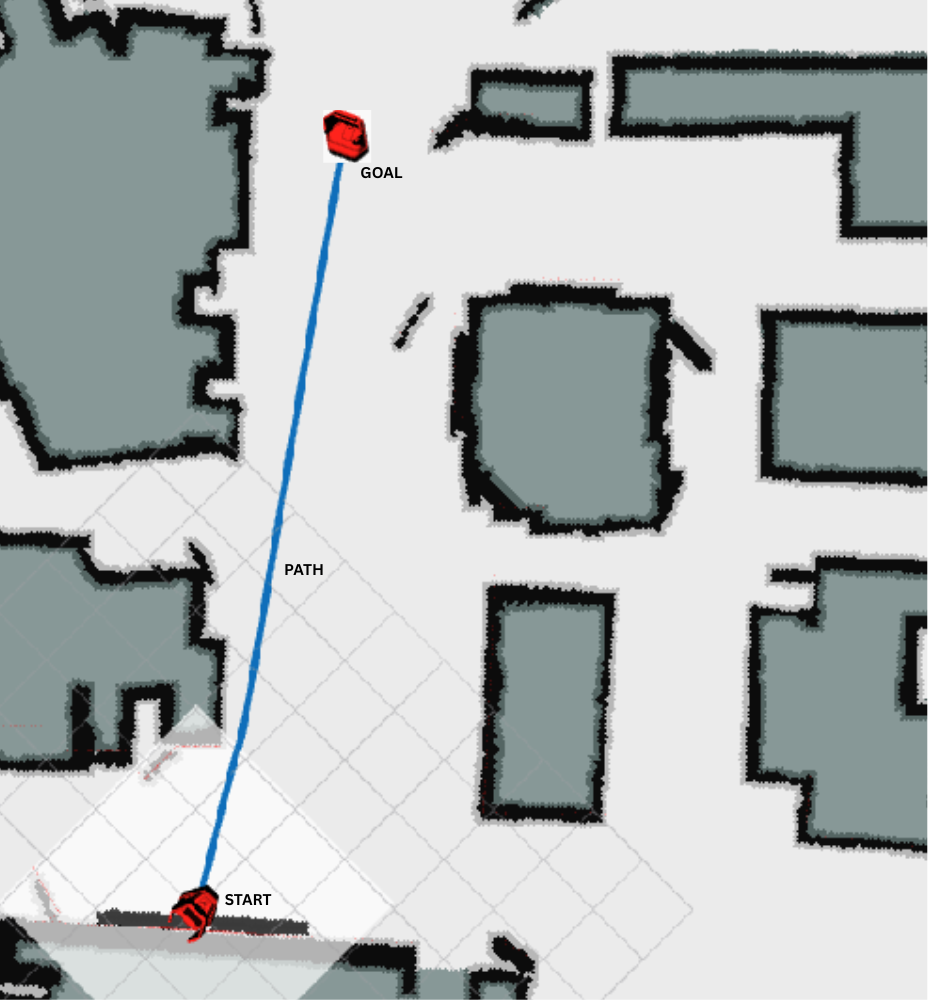
\includegraphics[width=\textwidth]{gambar/3.8_map_rviz.png}
        \\(b) Representasi RViz
    \end{minipage}
    \caption{Konfigurasi titik awal (START) dan tujuan (GOAL) yang identik untuk seluruh delapan skenario pengujian. (a) Tampak atas pada simulator Gazebo, menunjukkan kompleksitas geometris lingkungan \textit{indoor}. (b) Representasi pada RViz menggunakan peta \texttt{grit\_1\_edited\_2} (\textit{occupancy grid}), dengan garis biru menunjukkan jalur global yang dihasilkan NavfnROS sebelum eksekusi \textit{trial}. Koordinat \textit{frame} peta: START $= (0, 0)$, GOAL $= (9{,}159;\ 6{,}240)$.}
    \label{fig:map_annotated}
\end{figure}

Pada seluruh skenario, posisi awal robot ditetapkan pada koordinat yang sama, sedangkan posisi tujuan ditentukan pada titik akhir koridor navigasi. Dengan konfigurasi tersebut, seluruh percobaan dilakukan pada kondisi awal yang identik sehingga hasil pengujian dapat dibandingkan secara adil.

\subsection{Konfigurasi Baseline dan Fuzzy}

Konfigurasi baseline (S1--S4) menggunakan APFPlanner dengan parameter navigasi yang bersifat tetap. Pada konfigurasi ini, kecepatan robot dan penguatan gaya tolak obstacle dihitung menggunakan parameter bawaan APF tanpa mekanisme adaptasi.

Sebaliknya, konfigurasi fuzzy (S5--S8) menggunakan pengendali fuzzy Mamdani yang telah dijelaskan pada Subbab~\ref{sec:fuzzy_Aapf}. Nilai traversability efektif dan jarak obstacle terdekat digunakan sebagai masukan fuzzy untuk menghasilkan parameter \textit{speed scale} dan \textit{repulsive gain} secara adaptif.

Perbedaan utama kedua konfigurasi dirangkum pada Tabel~\ref{tab:konfigurasi_eksperimen}.

\begin{table}[H]
\centering
\caption{Perbandingan konfigurasi eksperimen}
\label{tab:konfigurasi_eksperimen}
\begin{tabular}{lll}
\toprule
\textbf{Komponen} &
\textbf{Baseline} &
\textbf{Fuzzy} \\
\midrule
LiDAR & Aktif & Aktif \\
Kamera termal & Aktif & Aktif \\
Virtual LaserScan & Aktif & Aktif \\
Fusi traversability & Aktif & Aktif \\
APFPlanner & Aktif & Aktif \\
Fuzzy Mamdani & Tidak aktif & Aktif \\
\bottomrule
\end{tabular}
\end{table}

\subsection{Prosedur Pelaksanaan Eksperimen}

Setiap skenario dieksekusi sebanyak sepuluh kali percobaan independen untuk memperoleh hasil yang lebih representatif dan mengurangi pengaruh variasi acak selama simulasi. Jumlah replikasi tersebut dipilih agar data yang diperoleh mencukupi untuk analisis statistik nonparametrik pada tahap evaluasi.

Urutan pelaksanaan eksperimen ditunjukkan pada Gambar~\ref{fig:prosedur_pengujian}.

\begin{figure}[H]
\centering
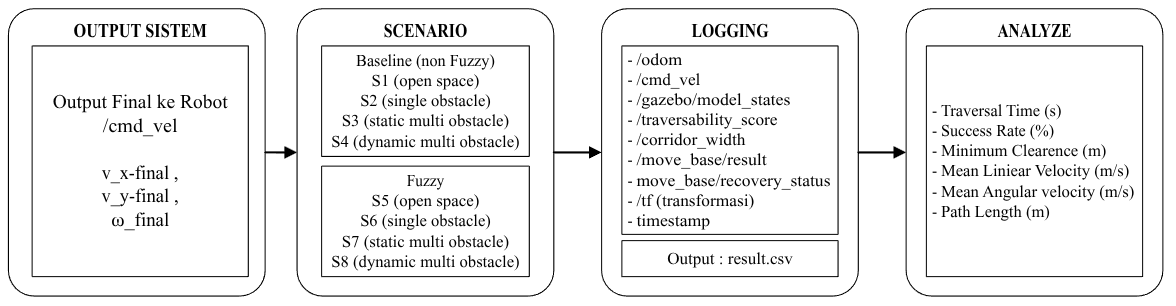
\includegraphics[width=0.9\textwidth]{gambar/3.8_prosedur_pengujian.png}
\caption{Alur pelaksanaan eksperimen.}
\label{fig:prosedur_pengujian}
\end{figure}

Secara umum, prosedur pengujian dilakukan melalui langkah-langkah berikut:

\begin{enumerate}
\item Menjalankan lingkungan simulasi Gazebo dan ROS.
\item Memuat peta navigasi dan model robot.
\item Mengaktifkan sensor LiDAR dan kamera termal.
\item Menjalankan modul navigasi sesuai konfigurasi pengujian.
\item Menetapkan posisi awal dan tujuan robot.
\item Menjalankan simulasi hingga robot mencapai tujuan atau eksperimen dihentikan.
\item Menyimpan seluruh data hasil eksperimen.
\item Mengulangi proses untuk seluruh skenario dan seluruh replikasi.
\end{enumerate}

\subsection{Pencatatan Data Eksperimen}

Selama eksperimen berlangsung, seluruh data dicatat secara otomatis menggunakan node \texttt{experiment\_logger.py}. Pencatatan dilakukan untuk memastikan seluruh informasi yang diperlukan pada tahap evaluasi tersedia secara lengkap dan konsisten.

Data yang direkam meliputi:

\begin{itemize}
\item posisi dan orientasi robot (\texttt{/odom}),
\item kecepatan linear dan angular (\texttt{/cmd\_vel}),
\item nilai traversability efektif,
\item jarak obstacle terdekat,
\item status pencapaian tujuan,
\item waktu pelaksanaan eksperimen.
\end{itemize}

Seluruh data disimpan dalam format CSV sehingga dapat digunakan untuk proses analisis statistik pada tahap berikutnya.